\documentclass[10pt,a4paper]{amsart}
\usepackage[margin=19mm]{geometry}
\usepackage{amsmath,amssymb,mathtools}
\usepackage[scr=rsfs,cal=euler]{mathalfa}
\usepackage{xfrac}
\usepackage[unicode,hidelinks,bookmarks=false]{hyperref}
\newcommand{\ie}{i.e.\ }
\newcommand{\cf}{cf.\ }
\newcommand{\resp}{respectively\ }
\newcommand{\Subsection}{\subsection}
\providecommand{\nobreakdash}{\nobreak\hbox{-}}
\setlength{\emergencystretch}{2em}
\multlinegap0pt
\usepackage{tikz}
\usepackage{tikz-cd}
\usepackage{graphicx}
\usetikzlibrary{arrows,calc,positioning,decorations.pathreplacing,cd}
\numberwithin{equation}{section}
\newcommand{\Emb}{\mathrm{Emb}}
\newcommand{\Diff}{\mathrm{Diff}}
\newcommand{\Aut}{\mathrm{Aut}}
\newcommand{\Map}{\mathrm{Map}}
\newcommand{\cat}{\ensuremath{\mathrm{Cat}}}
\newcommand{\topo}{\ensuremath{\mathrm{Top}}}
\newcommand{\obj}{\ensuremath{\mathrm{ob}}}
\newcommand{\pr}{\ensuremath{\mathrm{pr}}}
\newcommand{\opp}{\ensuremath{\mathrm{op}}}
\newcommand{\fib}{\ensuremath{\mathsf{fib}}}
\newcommand{\id}{\mathrm{id}}
\newcommand{\ab}{\mathrm{ab}}
\newcommand{\BM}{\mathrm{BM}}
\newcommand{\MCG}{\mathrm{MCG}}
\newcommand{\rincl}{\mathrm{incl}}

\newcommand{\Int}{\mathring}
\newcommand{\rgM}{\mathring{M}}
\newcommand{\tw}{\mathrm{tw}}
\newcommand{\colim}{\mathrm{colim}}
\newcommand{\Mot}{\mathrm{Mot}}
\newcommand{\mt}{\mathrm{t}}
\newcommand{\Aalg}{\ensuremath{\mathbb{A}\text{-}\mathrm{Alg}}}
\newcommand{\Rings}{\ensuremath{\mathrm{Rings}}}
\newcommand{\groups}{\ensuremath{\mathrm{Grp}}}
\newcommand{\triv}{\mathrm{tr}}
\newcommand{\col}{\mathrm{col}}
\newcommand{\unt}{\mathrm{u}}
\newcommand{\im}{\mathrm{Im}}
\newcommand{\Sp}{\mathrm{Sp}}
\newcommand{\rdec}{\mathrm{dec}}
\newcommand{\runl}{\mathrm{unl}}
\newcommand{\rface}{\mathrm{face}}
\newcommand{\rec}{\mathrm{ec}}
\newcommand{\rcoinv}{\mathrm{coinv}}
\newcommand{\rconj}{\mathrm{conj}}
\newcommand{\rStab}{\mathrm{Stab}}

%%%%%%%%%%%%%%%%%%%%%%%%%%%%%%%%%%


\newcommand{\mbar}{\ensuremath{{\,\,\overline{\!\! M\!}\,}}}
\newcommand{\nbar}{\ensuremath{{\,\,\overline{\!\! N}}}}

\newcommand{\B}{\ensuremath{\mathbf{B}}}
\newcommand{\MCGo}{\mathbf{\Gamma}}
\newcommand{\bn}{\mathbf{n}}
\newcommand{\lB}{\mathbf{LB}}
\newcommand{\fG}{\mathbf{G}}
\newcommand{\zero}{\mathbf{0}}


\newcommand{\MCGno}{\boldsymbol{\mathcal{N}}}
\newcommand{\LCS}{\varGamma}

\newcommand{\Sym}{\mathfrak{S}}
\newcommand{\LB}{\mathfrak{LB}}
\newcommand{\fF}{\mathfrak{F}}
\newcommand{\fU}{\ensuremath{\mathfrak{U}}}
\newcommand{\fkG}{\mathfrak{G}}
\newcommand{\fkc}{\mathfrak{c}}


\newcommand{\sR}{\mathscr{R}}
\newcommand{\sL}{\mathscr{L}}
\newcommand{\sF}{\mathscr{F}}
\newcommand{\sS}{\mathscr{S}}
\newcommand{\sB}{\mathscr{B}}
\newcommand{\N}{\mathscr{N}}



\newcommand{\tF}{\mathtt{F}}
\newcommand{\eF}{\mathsf{F}}
\newcommand{\sG}{\mathsf{G}}
\newcommand{\sC}{\mathsf{C}}
\newcommand{\sI}{\mathsf{i}}
\newcommand{\sr}{\mathsf{r}}

\newcommand{\cB}{\mathcal{B}}
\newcommand{\cC}{\mathcal{C}}
\newcommand{\cD}{\mathcal{D}}
\newcommand{\cE}{\mathcal{E}}
\newcommand{\cF}{\mathcal{F}}
\newcommand{\cG}{\mathcal{G}}
\newcommand{\cH}{\mathcal{H}}
\newcommand{\cL}{\mathcal{L}}
\newcommand{\cM}{\mathcal{M}}
\newcommand{\cO}{\mathcal{O}}
\newcommand{\cP}{\mathcal{P}}
\newcommand{\cQ}{\mathcal{Q}}
\newcommand{\cT}{\mathcal{T}}
\newcommand{\cU}{\mathcal{U}}
\newcommand{\cV}{\mathcal{V}}

\newcommand{\bA}{\mathbb{A}}
\newcommand{\bB}{\mathbb{B}}
\newcommand{\bD}{\mathbb{D}}
\newcommand{\bN}{\mathbb{N}}
\newcommand{\bR}{\mathbb{R}}
\newcommand{\bS}{\mathbb{S}}
\newcommand{\bZ}{\mathbb{Z}}


\newcommand{\longtwoheadrightarrow}{\longrightarrow\mathrel{\mkern-14mu}\rightarrow}
\newcommand{\longhookrightarrow}{\lhook\joinrel\longrightarrow}
\newcommand{\too}{\ensuremath{\longrightarrow}}


\newcommand{\diffdec}{\ensuremath{\mathrm{Diff}_{\rdec}}}
\newcommand{\diffdecbr}{\ensuremath{\mathrm{Diff}_{\rdec}^{\mathrm{br}}}}
%\newcommand{\diffbr}{\ensuremath{\mathrm{Diff}^{\mathrm{br}}}}
\newcommand{\diffdecbrplus}{\ensuremath{\mathrm{Diff}_{\rdec}^{\mathrm{br},+}}}
\newcommand{\diffdece}{\ensuremath{\mathrm{Diff}_{\rdec,\epsilon}}}
\newcommand{\diffdeceprime}{\ensuremath{\mathrm{Diff}_{\rdec,\epsilon'}}}
\newcommand{\diffdecet}{\ensuremath{\mathrm{Diff}_{\rdec,\epsilon,t}}}
\newcommand{\diffdecetprime}{\ensuremath{\mathrm{Diff}_{\rdec,\epsilon',t'}}}
\newcommand{\embdec}{\ensuremath{\mathrm{Emb}_{\rdec}}}
\newcommand{\embdece}{\ensuremath{\mathrm{Emb}_{\rdec,\epsilon}}}
\newcommand{\cdec}{\ensuremath{C^\infty_{\rdec}}}
\newcommand{\embgm}{\ensuremath{\mathrm{Emb}_{\langle \cG,\cM \rangle}}}
\newcommand{\Beta}{\boldsymbol{\beta}}



\NewDocumentCommand{\covlr}{O{\bullet} O{\bullet}}{
\ensuremath{{}_{#1}\mathrm{Cov}_{#2}} }
\NewDocumentCommand{\covl}{O{\bullet}}{
\ensuremath{{}_{#1}\mathrm{Cov}} }
\NewDocumentCommand{\covr}{O{\bullet}}{
\ensuremath{\mathrm{Cov}_{#1}} }
\NewDocumentCommand{\toplr}{O{\bullet} O{\bullet}}{
\ensuremath{{}_{#1}\mathrm{Top}_{#2}} }
\NewDocumentCommand{\topl}{O{\bullet}}{
\ensuremath{{}_{#1}\mathrm{Top}} }
\NewDocumentCommand{\topr}{O{\bullet}}{
\ensuremath{\mathrm{Top}_{#1}} }
\NewDocumentCommand{\modlr}{O{\bullet} O{\bullet}}{
\ensuremath{{}_{#1}\mathrm{Mod}_{#2}} }
\NewDocumentCommand{\modl}{O{\bullet}}{
\ensuremath{{}_{#1}\mathrm{Mod}} }
\NewDocumentCommand{\modr}{O{\bullet}}{
\ensuremath{\mathrm{Mod}_{#1}} }
\NewDocumentCommand{\topmodlr}{O{\bullet} O{\bullet} O{\bullet}}{
\ensuremath{{}_{#1}\mathrm{Top}_{#2}\mathrm{Mod}_{#3}} }
\NewDocumentCommand{\topmodlrpr}{O{\bullet} O{\bullet} O{\bullet}}{
\ensuremath{{}_{#1}\mathrm{Top}^{\mathrm{pr}}_{\,\, #2}\mathrm{Mod}_{#3}} }
\NewDocumentCommand{\topmodl}{O{\bullet} O{\bullet}}{
\ensuremath{{}_{#1}\mathrm{Top}_{#2}\mathrm{Mod}} }
\NewDocumentCommand{\topmodr}{O{\bullet} O{\bullet}}{
\ensuremath{\mathrm{Top}_{#1}\mathrm{Mod}_{#2}} }
\NewDocumentCommand{\setlr}{O{\bullet} O{\bullet}}{
\ensuremath{{}_{#1}\mathrm{Set}_{#2}} }
\NewDocumentCommand{\setl}{O{\bullet}}{
\ensuremath{{}_{#1}\mathrm{Set}} }



%\newcommand{\cA}{\mathcal{A}}
%\newcommand{\cI}{\mathcal{I}}
%\newcommand{\cJ}{\mathcal{J}}
%\newcommand{\cK}{\mathcal{K}}
%\newcommand{\cN}{\mathcal{N}}
%\newcommand{\cR}{\mathcal{R}}
%\newcommand{\cS}{\mathcal{S}}
%\newcommand{\cW}{\mathcal{W}}
%\newcommand{\cX}{\mathcal{X}}
%\newcommand{\cY}{\mathcal{Y}}
%\newcommand{\cZ}{\mathcal{Z}}
%\newcommand{\bC}{\mathbb{C}}


%\newcommand{\bE}{\mathbb{E}}
%\newcommand{\bF}{\mathbb{F}}
%\newcommand{\bG}{\mathbb{G}}
%\newcommand{\bH}{\mathbb{H}}
%\newcommand{\bI}{\mathbb{I}}
%\newcommand{\bJ}{\mathbb{J}}
%\newcommand{\bK}{\mathbb{K}}
%\newcommand{\bL}{\mathbb{L}}
%\newcommand{\bM}{\mathbb{M}}
%\newcommand{\bO}{\mathbb{O}}
%\newcommand{\bP}{\mathbb{P}}
%\newcommand{\bQ}{\mathbb{Q}}
%\newcommand{\bT}{\mathbb{T}}
%\newcommand{\bU}{\mathbb{U}}
%\newcommand{\bV}{\mathbb{V}}
%\newcommand{\bW}{\mathbb{W}}
%\newcommand{\bX}{\mathbb{X}}
%\newcommand{\bY}{\mathbb{Y}}

\renewcommand{\geq}{\geqslant}
\renewcommand{\leq}{\leqslant}

\newcommand{\incl}[3][right]
{
\draw[<-,>=#1 hook] #2 to ($ #2!0.5!#3 $);
\draw[->] ($ #2!0.5!#3 $) to #3;
}

%\newenvironment{itemizeb} {
%\begin{compactitem}
%\renewcommand{\labelitemi}{\ensuremath{\bullet}}
%\renewcommand{\labelitemii}{\ensuremath{\bullet}}} {
%\end{compactitem}}



\newcounter{stepcount}
\newenvironment{step}[1]{\refstepcounter{stepcount}\begin{proof}
[\textbf{Step~\thestepcount}]}{\let\qed\relax\end{proof}}
\newcommand*{\mk}{\mkern -1mu}
\newcommand*{\Mk}{\mkern -2mu}
\newcommand*{\mK}{\mkern 1mu}
\newcommand*{\MK}{\mkern 2mu}
\newcommand*{\romanenumi}{\renewcommand*{\theenumi}{\roman{enumi}}}
\newcommand*{\bromanenumi}{\renewcommand*{\theenumi}{\textbf{\roman{enumi}}}}
\newcommand*{\Romanenumi}{\renewcommand*{\theenumi}{\Roman{enumi}}}
\newcommand*{\alphenumi}{\renewcommand*{\theenumi}{\alph{enumi}}}
\newcommand*{\Alphenumi}{\renewcommand*{\theenumi}{\Alph{enumi}}}
\let\oldtilde\tilde
\renewcommand*{\tilde}[1]{\mathchoice{\widetilde{#1}}{\widetilde{#1}}{\oldtilde{#1}}{\oldtilde{#1}}}
\let\oldhat\hat
\renewcommand*{\hat}[1]{\mathchoice{\widehat{#1}}{\widehat{#1}}{\oldhat{#1}}{\oldhat{#1}}}
\let\oldexists\exists
\renewcommand*{\exists}{\mathrel{\oldexists}}
\newtheorem{theo}{Theorem}[section]
\newtheorem{prop}[theo]{Proposition}
\newtheorem{lemm}[theo]{Lemma}
\newtheorem{coro}[theo]{Corollary}
\theoremstyle{definition}
\newtheorem{defi}[theo]{Definition}
\newtheorem{nota}[theo]{Notation}
\newtheorem{notation}[theo]{Notation}
\newtheorem{construction}[theo]{Construction}
\theoremstyle{remark}
\newtheorem{rema}[theo]{Remark}
\newenvironment{enonce}[1]{\begin{construction}}{\end{construction}}
\title[Serre fibration for unoriented decorated boundary sums]{Serre fibration and embedding-space quotient identification for unoriented decorated boundary sums in dimensions at least two other than four}
\author{Martin Palmer and Arthur Souli\'e}
\date{Source: Annales Henri Lebesgue \textbf{7} (2024), 409--520; DOI 10.5802/ahl.204; official published version}
\begin{document}
\maketitle
\noindent\textit{Editorial scope.} The counted unit is the first (unoriented) assertion of original Theorem 1.55 together with its complete authored proof, including the local retraction construction and the four extension steps. Retained uncounted core: the publisher-native definitions of morphisms and morphism spaces of decorated manifolds, the lemmas on open path-components and on the decomposition of decorated embedding spaces, the definition of decorated embeddings with Notation 1.50, and the two authored figures of the proof, all copied exactly from the source. The published dimension restriction $d\neq 4$ and the published numbering are reproduced.\par
\noindent\textit{Reference handling and bounded omissions.} Two purely navigational clauses were removed and are listed verbatim in the machine-readable fidelity receipt: the forward-pointing opening of \S 1.3 (which announces downstream sections of the published article) and the trailing list of downstream subsections inside Remark 1.54. Every hypothesis, definition, formula, construction and conclusion is retained unchanged; the $d\neq 4$ assumption itself and its stated reason are kept in full.
\section{Categories of decorated manifolds and their embeddings}\label{s:categorical_framework}

\subsection{Decorated manifolds and their diffeomorphisms}\label{ss:topological_groupoids_of_decorated_manifolds}

\setcounter{theo}{2}
\begin{lemm}\label{lem:open-path-components}
If $X$ has the property that its path-components are open, then the quotient space $X/{\sim}$ also has this property, for any equivalence relation $\sim$ on $X$. If a collection~$X_i$ of spaces all have this property, then so does their disjoint union $\bigsqcup_i X_i$.
\end{lemm}

There is a canonical way to refine the topology on an arbitrary space in order to force this property to hold.

\begin{enonce}{Construction}\label{construction:open-path-components}
For a topological space $X$, denote by $o(X)$ the topological space with the same underlying set as $X$, equipped with the topology generated by the base consisting of $C \cap U$ for $U$ an open subset of $X$ and $C$ a path-component of~$X$.
\end{enonce}

One may easily verify the following properties of this construction.

\begin{lemm}\label{lem:properties-of-o}
The path-components of $o(X)$ are open, and they are the same as the path-components of $X$. The canonical map $o(X) \to X$ defined by the identity map of the underlying sets is continuous, and becomes a homeomorphism when restricted to any path-component. Consequently, it is also a weak equivalence. In addition, the functor $o(-)$ preserves products.
\end{lemm}

\begin{rema}\label{rmk:coreflective-subcategory}
In fact, the operation $o(-)$ is a right adjoint to the inclusion of the full subcategory of topological spaces having the property that their path-components are open; this subcategory is therefore \emph{coreflective}.
\end{rema}

Finally, we will need the following lemma, which explains how the operation $o(-)$ interacts with quotient maps that are Serre fibrations.

\begin{lemm}\label{lem:open-path-components-Serre-fibrations}
Let $X$ be a topological space and $\sim$ an equivalence relation on $X$. If the quotient map $X \to X/{\sim}$ is a Serre fibration, then so is the quotient map $o(X) \to o(X)/{\sim}$.
\end{lemm}

\begin{proof}
The continuous bijection $o(X) \to X$ induces a continuous bijection $o(X)/{\sim} \to X/{\sim}$, fitting into a commutative square with the two quotient maps. Let us consider the lifting problem:


\begin{equation}\label{eq:lifting-problem-o}
\begin{tikzcd}
{[0,1]^{d-1}} \ar[rr] \ar[d] && o(X) \ar[d] \ar[r] & X \ar[d] \\
{[0,1]^d} \ar[rr] \ar[densely dashed,rru,"?"] && o(X)/{\sim} \ar[r] & X/{\sim}.
\end{tikzcd}
\end{equation}
Since $X \to X/{\sim}$ is a Serre fibration by hypothesis, there is a diagonal map $[0,1]^d \to X$ making the two outer triangles commute. Since the cube $[0,1]^d$ is path-connected, its image in $X$ lies in a single path-component. Restricted to this path-component, the continuous bijection $o(X) \to X$ is a homeomorphism by Lemma~\ref{lem:properties-of-o}, so we may lift the diagonal map $[0,1]^d \to X$ to a diagonal map $[0,1]^d \to o(X)$ for the left-hand square, as desired. The two triangles into which this splits the left-hand square of~\eqref{eq:lifting-problem-o} commute, since the triangles that the outer rectangle was split into commute and the two right-hand horizontal maps in~\eqref{eq:lifting-problem-o} are bijective.
\end{proof}

\begin{rema}
Lemma~\ref{lem:open-path-components-Serre-fibrations} holds more generally for any class of fibrations defined by the right lifting property with respect to a collection of maps whose codomains are path-connected. Moreover, it also holds more generally for any two topologies on the same underlying set that have the same path-components and that agree on each path-component.
\end{rema}


\setcounter{theo}{11}
\begin{defi}[Morphisms of decorated manifolds.]\label{def:decorated-manifolds-morphisms}
A morphism of decorated manifolds from $(M,A,e_{1},e_{2})$ to $(M',A',e'_{1},e'_{2})$ is a smooth, proper (preimages of compact subspaces are compact) map $\varphi \colon M \to M'$ such that $\varphi(A) \subseteq A'$ and such that, for some $\epsilon > 0$ and for each $i \in \{1,2\}$, we have $\varphi(e_{i}(\bB^d_\epsilon)) = e'_{i}(\bB^d_\epsilon)$ and the composition $(e'_{i})^{-1} \circ \varphi \circ e_{i} \colon \bB^d_\epsilon \rightarrow \bB^d_\epsilon$ is the identity. Write $C^\infty_{\rdec}(M,M')$ for the set of such morphisms, where by abuse of notation we are abbreviating $(M,A,e_{1},e_{2})$ to $M$ and $(M',A',e'_{1},e'_{2})$ to $M'$.
\end{defi}

For decorated manifolds $M$ and $M'$, we equip the set $C^\infty_{\rdec}(M,M')$ with a topology induced by a colimit of Whitney topologies, as follows.
\begin{itemize}
\item Choose representative boundary cylinders for the boundary-cylinder germs $e_{i}$ and $e'_{i}$. This ensures that the condition in Definition~\ref{def:decorated-manifolds-morphisms} makes sense for a fixed $\epsilon \in (0,1)$, not just for an unspecified $\epsilon \in (0,1)$ that is quantified over.
\item Fix $\epsilon \in (0,1)$ and write $C^\infty_{\rdec,\epsilon}(M,M')$ for the subset of $C^\infty_{\rdec}(M,M')$ where the condition in Definition~\ref{def:decorated-manifolds-morphisms} holds for this fixed $\epsilon$. Equip each subset $C^\infty_{\rdec,\epsilon}(M,M')$ with the subspace topology induced from the smooth Whitney topology on the set $C^\infty(M,M')$ of \emph{all} smooth maps from $M$ to $M'$; for details of the Whitney topology, see for example~\cite[Chap.~2]{Hirsch1976Differentialtopology}. As a set, note that $C^\infty_{\rdec}(M,M')$ is the union of $C^\infty_{\rdec,\epsilon}(M,M')$ over all choices of $\epsilon \in (0,1)$.
\end{itemize}

\begin{lemm}\label{lem:topology_well_defined}
The colimit topology determined by the increasing filtration $\{ C^\infty_{\rdec,\epsilon}(M,M') \}_{\epsilon\,\in\,(0,1)}$ does not depend on the choices of representative boundary-cylinders for the boundary-cylinder germs $e_{i}$ and $e'_{i}$.
\end{lemm}

\begin{proof}
Different choices of representative boundary-cylinders for the boundary-cylinder germs $e_{i}$ and $e'_{i}$ result in different filtrations, which are cofinal in each other, so the induced colimit topologies are equal.
\end{proof}

\begin{defi}[Morphism spaces.]\label{def:decorated-manifolds-morphism-spaces}
The morphism set $C^\infty_{\rdec}(M,M')$ is topologised as follows: we first consider the colimit topology induced by the increasing filtration $\{ C^\infty_{\rdec,\epsilon}(M,M') \}_{\epsilon\,\in\,(0,1)}$ and then we apply the functor $o(-)$ of Construction~\ref{construction:open-path-components} to ensure that all path-components are open. Thus we may write
\[
C^\infty_{\rdec}(M,M') := o\left(\underset{\epsilon\,\to\,0}{\colim}(C^\infty_{\rdec,\epsilon}(M,M'))\right).
\]
\end{defi}

We note that composition is continuous in this topology since the functor $o(-)$ preserves products (by Lemma~\ref{lem:properties-of-o}) and because composition of smooth, proper maps is continuous in the Whitney topology (see~\cite[\S~2, Prop.~1]{Mather1969}).

\begin{rema}
Depending on $M$ and $M'$, the topology of Definition~\ref{def:decorated-manifolds-morphism-spaces} may differ from the subspace topology inherited directly from the Whitney topology on $C^\infty(M,M')$: the colimit topology is in general finer than the directly inherited Whitney topology, and the operation $o(-)$ refines the topology further. However, these three topologies on $\cdec(M,M')$ are all weakly equivalent (see Lemma~\ref{lem:properties-of-o}). In particular, they have the same $\pi_{0}$.
\end{rema}

We can now introduce the topologically-enriched categories associated to decorated manifolds:


\setcounter{theo}{48}
\subsection{A Serre fibration of decorated diffeomorphism groups}\label{ss:fibration-condition}

\emph{From this point onwards, we assume that the dimension $d$ is not equal to $4$}; see Remark~\ref{rmk:d_neq_4_explanation} for the reason why this is necessary. We start by introducing the following notion.


\begin{defi}[Decorated embeddings.]\label{def:embdec}
Let $M = (M,A)$ and $N = (N,B)$ be decorated manifolds. Define $\embdec(M,N)$ to be the set of smooth, proper embeddings $\varphi \colon M \hookrightarrow N$, equipped with a germ of an extension $\varphi'$ to an embedding $\bB_{1}^d \natural M \hookrightarrow N$, such that:
\begin{itemize}
\item $\varphi(A) \subseteq B$;
\item for some $\epsilon > 0$ we have $\varphi(e_{2}(\bB_{\epsilon}^d)) = e'_{2}(\bB_{\epsilon}^d)$ and $(e'_{2})^{-1} \circ \varphi \circ e_{2}$ is the identity map $\bB_{\epsilon}^d \to \bB_{\epsilon}^d$, where $e_{1},e_{2}$ are the boundary-cylinder germs of $(M,A)$ and $e'_{1},e'_{2}$ are those of $(N,B)$;
\item there is a decorated manifold $M'$ and diffeomorphism of decorated manifolds $\bar{\varphi} \colon M' \natural M \to N$ such that $\varphi = \bar{\varphi} \circ \iota_{M,M'}$, where $\iota_{M,M'}$ denotes the canonical embedding of $M$ into $M' \natural M$. This extension of $\varphi$ to $\bar{\varphi}$ should be compatible with the given germ of an extension $\varphi'$ of $\varphi$.
\end{itemize}
In other words -- modulo decorated diffeomorphisms of the codomain -- a decorated embedding is the canonical inclusion of (a germ of a neighbourhood of) the right-hand factor of a boundary connected sum. As an illustration, Figure~\ref{fig:decorated-manifolds-Mt} depicts the inclusion of a neighbourhood $M_t$ of $M$ into $L\natural M$, representing a decorated embedding of $M$ into $L\natural M$.

We now describe the topology on this set. Recall that $\mbar = \bB^d_1 \natural M = (\bD^{d-1} \times [-1,0]) \cup M$ and write $M_t = (\bD^{d-1} \times [-t,0]) \cup M$ for $t \in (0,1)$, as depicted in Figure~\ref{fig:decorated-manifolds-Mt}. For $\epsilon \in (0,1)$, write $\embdece(M_t,N)$ for the set of embeddings defined as above except that $\epsilon$ is fixed in the second bullet point and the embedding is defined on $M_t$ rather than on $M$ plus a germ of a neighbourhood. Topologise $\embdece(M_t,N)$ as a subspace of $C^\infty(M_t,N)$ equipped with the Whitney topology. We may take the colimit as $\epsilon \to 0$ (along inclusion maps) and $t \to 0$ (along restriction maps), and we define $\embdec(M,N) := o(\underset{\epsilon,t\,\to\,0}{\colim}(\embdece(M_t,N)))$, where $o(-)$ is the functor of Construction~\ref{construction:open-path-components}.
\end{defi}

\begin{nota}\label{notation:decorated-embeddings}
For decorated manifolds $L,M,N$, we denote by $\embdec(M,N)_L$ the subspace of $\embdec(M,N)$ of those embeddings for which we may take $M' = L$ in the third point above. Additionally, if $A$ and $B$ are oriented, we denote by $\embdec^{+}(M,N)$ the subspace of $\embdec(M,N)$ of those decorated embeddings $\varphi \colon M \hookrightarrow N$ whose restriction $\varphi|_A \colon A \hookrightarrow B$ is orientation-preserving.
\end{nota}

The composition of decorated embeddings is defined as follows.

\begin{defi}\label{def:decorated-embeddings-composition}
Let $\varphi\in\embdec(M,N)$ and $\psi\in\embdec(N,P)$ for decorated manifolds $M$, $N$ and $P$. Choose decorated diffeomorphisms $\bar{\varphi} \colon M' \natural M \to N$ and $\bar{\psi} \colon N' \natural N \to P$ extending $\varphi$ and $\psi$ respectively; these exist by definition. We may then form the composite decorated diffeomorphism $\bar{\psi} \circ (\id_{N'} \natural \bar{\varphi}) \colon N' \natural M' \natural M \to P$, which restricts to the composite embedding $\psi \circ \varphi$ on $M \subset N' \natural M' \natural M$. Moreover, its restriction to an $\epsilon$-neighbourhood of $M \subset N' \natural M' \natural M$ provides a germ of an extension of $\psi \circ \varphi$ to $\bB_{1}^d \natural M$. The first two points of Definition~\ref{def:embdec} clearly hold for the composite embedding $\psi \circ \varphi$, so this embedding together with the germ of an extension is an element of $\embdec(M,P)$, which we define to be the composition of the decorated embeddings $\varphi$ and $\psi$.
\end{defi}

\begin{lemm}\label{lem:decorated-embeddings-composition-continuous-associative}
The composition of decorated embeddings given in Defini\-tion \ref{def:decorated-embeddings-composition} defines a continuous, associative operation $\embdec(M,N) \times \embdec(N,P)\newline \to \embdec(M,P)$.
\end{lemm}

\begin{proof}
We must first check that this operation is a well-defined map, i.e.~that the construction of Definition~\ref{def:decorated-embeddings-composition} does not depend on the choice of decorated diffeomorphisms $\bar{\varphi}$ and $\bar{\psi}$ extending $\varphi$ and $\psi$. The only part of the construction that depends on these choices of extensions is the germ of an extension of $\psi \circ \varphi$ to an embedding $\bB_{1}^d \natural M \hookrightarrow P$. The fact that this germ is independent of the choice of decorated diffeomorphisms extending the decorated embeddings follows from the fact that decorated diffeomorphisms are required to be compatible with boundary-cylinder germs. Continuity of the operation follows from the fact that composition of proper, smooth maps is continuous in the Whitney topology; see~\cite[\S~2, Prop.~1]{Mather1969}.

Finally, let us check associativity of this operation. For $\varphi\in\embdec(M,N)$, $\psi\in\embdec(N,P)$ and $\chi\in\embdec(P,Q)$, the two iterated compositions $(\chi \circ \psi) \circ \varphi$ and $\chi \circ (\psi \circ \varphi) \in \embdec(M,Q)$ each consist of a smooth embedding $M \hookrightarrow Q$ and a germ of an extension to $\bB_{1}^d \natural M \hookrightarrow Q$. The two smooth embeddings $M \hookrightarrow Q$ are evidently equal, by associativity of composition of maps. Moreover, the fact that the two germs of extensions to embeddings $\bB_{1}^d \natural M \hookrightarrow Q$ are equal follows from the fact that they are restrictions, to an $\epsilon$-neighbourhood of $M \subset P' \natural N' \natural M' \natural M$, of the decorated diffeomorphisms $(\bar{\chi} \circ (\id_{P'} \natural \bar{\psi})) \circ (\id_{P' \natural N'} \natural \bar{\varphi})$ and $\bar{\chi} \circ ((\id_{P'} \natural \bar{\psi}) \circ (\id_{P' \natural N'} \natural \bar{\varphi}))$, which are equal by associativity of composition of maps.
\end{proof}

\begin{lemm}\label{lem:decomposition-disjoint-union}
The embedding space $\embdec(M,N)$ decomposes as a topological disjoint union
\begin{equation}\label{eq:embdec-decomposition}
\embdec(M,N) \;\cong\; \bigsqcup_L \, \embdec(M,N)_L,
\end{equation}
where the disjoint union runs over representatives of isomorphism classes of decorated manifolds.
\end{lemm}


\begin{proof}
We denote by $(-)^{\fkc}$ the function
\[
\embdec(M,N) \too \{ \text{isomorphism classes of decorated manifolds} \}
\]
that assigns to each decorated embedding the isomorphism class of the decorated manifold given by the complement of its image. We must show that this function is locally constant. Let $\varphi \in \embdec(M,N)$ be any decorated embedding; we must show that it admits a neighbourhood $\cU$ such that $\psi^{\fkc} = \varphi^{\fkc}$ for each $\psi \in \cU$.

Since $\varphi$ is a decorated embedding, we may fix an identification of $N$ with $L \natural M$, for some decorated manifold $L$, such that $\varphi$ is (the germ of an extension to a collar neighbourhood of) the canonical inclusion of $M$ into $L \natural M$.

We first note that there exists an open neighbourhood $\cU$ of $\varphi$ such that, for each $\psi \in \cU$, the interface $\psi(M) \cap (\overline{(L \natural M)) \smallsetminus \psi(M)})$ between the image of $\psi$ and its complement is a smoothly embedded $(d-1)$-dimensional disc $D(\psi)$ contained in the central solid cylinder $\bD^{d-1} \times [-1,1]$ along which the boundary connected sum of $L \natural M$ is formed; see Figure~\ref{fig:decorated-manifolds-Mt}. Moreover, $D(\psi)$ intersects the boundary of $\bD^{d-1} \times [-1,1]$ precisely in $\partial D(\psi)$. Such an open neighbourhood $\cU$ exists in the compact-open topology, and hence also in the topology that we are considering on $\embdec(M,N)$ (a refinement of a colimit of Whitney topologies), which is finer than the compact-open topology.

It remains to show, for a given $\psi \in \cU$, that $\psi^{\fkc} = \varphi^{\fkc}$. The embedded codimension-$1$ disc $D(\psi)$ cuts the solid cylinder $\bD^{d-1} \times [-1,1]$ into two pieces; let us denote by $A(\psi)$ the piece that contains $\bD^{d-1} \times \{-1\}$. We claim that $A(\psi)$ is diffeomorphic to $\bD^{d-1} \times [-1,0]$ by a diffeomorphism $\Xi$ that acts by the identity on a neighbourhood of $\bD^{d-1} \times \{-1\}$. This claim will immediately imply that $\psi^{\fkc} = \varphi^{\fkc}$, as desired, by extending $\Xi$ by the identity on $L \smallsetminus (\bD^{d-1} \times [-1,0])$.

Smoothing corners, we may rephrase the claim in the previous paragraph as follows. Consider the standard $d$-ball $\bD^d \subset \bR^d$, denote by $\bD^d_+$ the closed upper half-ball and fix a small $(d-1)$-dimensional subdisc $D_0$ of the boundary $\partial \bD^d$ centred at the north pole. Suppose we are given a smoothly embedded $(d-1)$-dimensional disc $D \subset \bD^d$ with $D \cap \partial \bD^d = \partial D$ disjoint from $D_0$ and denote by $A$ the closure of the component of $\bD^d \smallsetminus D$ containing $D_0$. The claim is that there exists a diffeomorphism $\Xi \colon A \cong \bD^d_+$ that acts by the identity on a neighbourhood of $D_0$. As explained above, this claim will complete the proof.

To prove this claim, we first consider the \emph{double} $2(\bD^d)$ of $\bD^d$, which is a smooth $d$-sphere. Smoothing corners again, the boundary of $A \subset \bD^d \subset 2(\bD^d)$ is a smoothly embedded $(d-1)$-sphere. The smooth Schoenflies theorem (see~\cite{Schoenflies1906} for $d=2$, see~\cite{Brown1960,Mazur1959,Morse1960} for $d=3$ and see~\cite[Prop.~D, \S~9]{Milnor1965} for $d\geq 5$) then implies that $A$ is diffeomorphic to a $d$-ball. Smoothing corners yet again, this gives a diffeomorphism $\Xi' \colon A \cong \bD^d_+$. However, this does not necessarily act by the identity on a neighbourhood of $D_0$.

To ensure this second condition, let $e \colon \bD^d \hookrightarrow \bD^d$ be an orientation-preserving embedding so that $e(\bD^d)$ is a neighbourhood of $D_0$ and so that $e(\bD^d)$ is contained in $A \cap \bD^d_+$. Then $e$ and $\Xi' \circ e$ are two embeddings of $\bD^d$ into $\bD^d_+$. By composing $\Xi'$ with a reflection if necessary, $\Xi' \circ e$ is also orientation-preserving. Palais' disc embedding theorem~\cite[Thm.~B]{Palais1960Extendingdiffeomorphisms} implies that there is a diffeomorphism $\Xi'' \colon \bD^d_+ \cong \bD^d_+$ such that $\Xi'' \circ e = \Xi' \circ e$. The composition $\Xi := (\Xi'')^{-1} \circ \Xi' \colon A \cong \bD^d_+$ is then a diffeomorphism that acts by the identity on the neighbourhood $e(\bD^d)$ of $D_0$, as desired.
\end{proof}

\begin{rema}\label{rmk:d_neq_4_explanation}
The proof above uses the smooth Schoenflies theorem, which is an open question (rather than a theorem) in dimension $d=4$; this is the reason for the restriction $d \neq 4$ that we make in the present subsection \S~\ref{ss:fibration-condition}\end{rema}

Now, for the remainder of \S~\ref{ss:fibration-condition}, we consider two decorated manifolds $L = (L,A,e_{1},e_{2})$ and $M = (M,B,e'_{1},e'_{2})$. There is a continuous right action of $\diffdec(L)$ on $\diffdec(L \natural M)$ given by $\varphi \cdot \psi = \varphi \circ (\psi \natural \id_M)$, and hence a quotient map

\setcounter{equation}{22}
\begin{equation}\label{eq:quotient-diff}
\Psi \colon \diffdec(L \natural M) \too \diffdec(L \natural M) / \diffdec(L).
\end{equation}


\begin{theo}\label{thm:fibre-bundle}
The quotient map~\eqref{eq:quotient-diff} is a Serre fibration. There is a homeomorphism between its codomain and $\embdec(M,L \natural M)_L$, induced by the restriction map.

If the submanifolds $A \subset \Int{L}$ and $B \subset \Int{M}$ are oriented and we consider the subgroups $\diffdec^{+}(-)$ of $\diffdec(-)$, then the analogue of the quotient map~\eqref{eq:quotient-diff} is also a Serre fibration and there is a homeomorphism from its codomain to $\embdec^{+}(M,L \natural M)_L$, induced by the restriction map.
\end{theo}


\begin{rema}
This is related to results of Cerf~\cite[p.~294, \S~II.2.2.2, Cor.~2]{Cerf1961Topologiedecertains}, Palais~\cite[Th.~B]{Palais1960Localtrivialityof} and Lima~\cite{Lima1963localtrivialityof}, but we were not able to find an instance of their results that covers exactly the setting that we need here. We therefore give a complete proof of Theorem~\ref{thm:fibre-bundle} below, using as an input two results of Cerf and Palais, namely~\cite[Lemme~II.2.1.2 (p.~291)]{Cerf1961Topologiedecertains} and~\cite[Th.~A]{Palais1960Localtrivialityof}.
\end{rema}

\setcounter{figure}{2}
\begin{figure}[t]
\centering
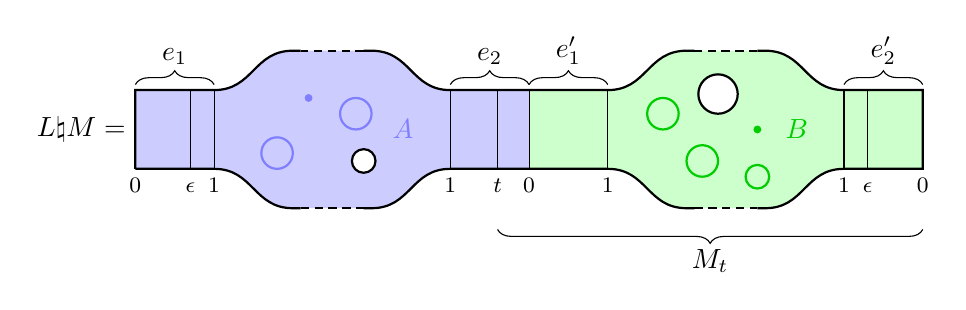
\begin{tikzpicture}
[x=1mm,y=1mm,scale=1]
\begin{scope}[xshift=5mm]
\fill[blue!20] (0,0) -- (10,0).. controls (15,0) and (15,-5).. (20,-5) -- (21,-5) -- (29,-5) -- (30,-5).. controls (35,-5) and (35,0).. (40,0) -- (50,0) -- (50,10) -- (40,10).. controls (35,10) and (35,15).. (30,15) -- (29,15) -- (21,15) -- (20,15).. controls (15,15) and (15,10).. (10,10) -- (0,10) -- cycle;
\draw[thick] (0,0) -- (10,0).. controls (15,0) and (15,-5).. (20,-5) -- (21,-5);
\draw[thick,densely dashed] (21,-5) -- (29,-5);
\draw[thick] (29,-5) -- (30,-5).. controls (35,-5) and (35,0).. (40,0) -- (50,0);
\draw[thick] (50,10) -- (40,10).. controls (35,10) and (35,15).. (30,15) -- (29,15);
\draw[thick,densely dashed] (29,15) -- (21,15);
\draw[thick] (21,15) -- (20,15).. controls (15,15) and (15,10).. (10,10) -- (0,10) -- (0,0);
\draw[blue!50,thick] (18,2) circle (2);
\draw[blue!50,thick] (28,7) circle (2);
\fill[blue!50,thick] (22,9) circle (0.5);
\node at (34,5) [blue!50] {$A$};
\fill[white] (29,1) circle (1.5);
\draw[thick] (29,1) circle (1.5);
\draw (7,0) -- (7,10);
\draw (10,0) -- (10,10);
\node at (0,0) [anchor=north,font=\footnotesize] {$0$};
\node at (7,0) [anchor=north,font=\footnotesize] {$\vphantom{0}\epsilon$};
\node at (10,0) [anchor=north,font=\footnotesize] {$1$};
\node at (5,12) [anchor=south] {$e_{1}$};
\draw[decorate,decoration={brace,amplitude=5pt,raise=2pt}] (0,10) -- (10,10);
\node at (0,5) [anchor=east] {$L \natural M =$};
\end{scope}
\begin{scope}[xshift=55mm]
\fill[green!20] (0,0) -- (10,0).. controls (15,0) and (15,-5).. (20,-5) -- (21,-5) -- (29,-5) -- (30,-5).. controls (35,-5) and (35,0).. (40,0) -- (50,0) -- (50,10) -- (40,10).. controls (35,10) and (35,15).. (30,15) -- (29,15) -- (21,15) -- (20,15).. controls (15,15) and (15,10).. (10,10) -- (0,10) -- cycle;
\draw[thick] (0,0) -- (10,0).. controls (15,0) and (15,-5).. (20,-5) -- (21,-5);
\draw[thick,densely dashed] (21,-5) -- (29,-5);
\draw[thick] (29,-5) -- (30,-5).. controls (35,-5) and (35,0).. (40,0) -- (50,0) -- (50,10) -- (40,10).. controls (35,10) and (35,15).. (30,15) -- (29,15);
\draw[thick,densely dashed] (29,15) -- (21,15);
\draw[thick] (21,15) -- (20,15).. controls (15,15) and (15,10).. (10,10) -- (0,10);
\draw[green!80!black,thick] (17,7) circle (2);
\draw[green!80!black,thick] (22,1) circle (2);
\draw[green!80!black,thick] (29,-1) circle (1.5);
\fill[green!80!black,thick] (29,5) circle (0.5);
\fill[white] (24,9.5) circle (2.5);
\draw[thick] (24,9.5) circle (2.5);
\node at (34,5) [green!80!black] {$B$};
\draw (40,0) -- (40,10);
\draw (43,0) -- (43,10);
\node at (40,0) [anchor=north,font=\footnotesize] {$1$};
\node at (43,0) [anchor=north,font=\footnotesize] {$\vphantom{0}\epsilon$};
\node at (50,0) [anchor=north,font=\footnotesize] {$0$};
\node at (45,12) [anchor=south] {$e'_{2}$};
\draw[decorate,decoration={brace,amplitude=5pt,raise=2pt}] (40,10) -- (50,10);
\draw (-10,0) -- (-10,10);
\draw (-4,0) -- (-4,10);
\draw (0,0) -- (0,10);
\draw (10,0) -- (10,10);
\node at (-10,0) [anchor=north,font=\footnotesize] {$1$};
\node at (-4,0) [anchor=north,font=\footnotesize] {$\vphantom{0}t$};
\node at (0,0) [anchor=north,font=\footnotesize] {$0$};
\node at (10,0) [anchor=north,font=\footnotesize] {$1$};
\draw[decorate,decoration={brace,amplitude=5pt,raise=2pt}] (-10,10) -- (0,10);
\draw[decorate,decoration={brace,amplitude=5pt,raise=2pt}] (0,10) -- (10,10);
\node at (-5,12) [anchor=south] {$e_{2}$};
\node at (5,12) [anchor=south] {$e'_{1}$};
\draw[decorate,decoration={brace,amplitude=5pt,mirror,raise=2pt}] (-4,-7) -- (50,-7);
\node at (23,-9) [anchor=north] {$M_t$};
\end{scope}
\end{tikzpicture}
\caption{The boundary connected sum $L \natural M$ from the proof of Theorem~\ref{thm:fibre-bundle}.}\label{fig:decorated-manifolds-Mt}
\end{figure}

\begin{proof}[Proof of Theorem~\ref{thm:fibre-bundle}]
In the proof below, we use the topology on the spaces of decorated diffeomorphisms and of decorated embeddings given by a colimit of Whitney topologies, as described in Definitions~\ref{def:decorated-manifolds-morphism-spaces} and~\ref{def:embdec}, thus proving that~\eqref{eq:quotient-diff} is a Serre fibration for this topology. This result automatically implies that the same result holds when using the finer topology making all path-components open; see Lemma~\ref{lem:open-path-components-Serre-fibrations}. Hence we shall make no further mention of this finer topology and work directly with the colimit of Whitney topologies.

Moreover, we detail here the proof for the first (unoriented) case of Theorem~\ref{thm:fibre-bundle}. All of the arguments below repeat mutatis mutandis in the setting where the submanifolds $A$ and $B$ are oriented and the morphisms of decorated manifolds preserve these orientations.

The decorated manifolds $L = (L,A,e_{1},e_{2})$ and $M = (M,B,e'_{1},e'_{2})$ come equipped with germs $e_{1},e_{2},e'_{1},e'_{2}$ of boundary cylinders; let us once and for all choose representative boundary cylinders for these germs, and denote them by the same symbols, by abuse of notation.

For $\epsilon \in (0,1)$, let $\diffdece(L\natural M)$ denote the group of self-diffeomorphisms of $L\natural M$ sending $A \sqcup B$ onto itself and restricting to the identity on $e_{1}(\bB_{\epsilon}^d)$ and on $e'_{2}(\bB_{\epsilon}^d)$. If we give this the Whitney topology, then we have
\begin{equation}\label{eq:diff-colimit-identification}
\diffdec(L\natural M) \cong \underset{\epsilon\,\to\,0}{\colim} (\diffdece(L\natural M)),
\end{equation}
by Definitions~\ref{def:decorated-manifolds-morphisms} and~\ref{def:decorated-manifolds-morphism-spaces} (recalling that, after the first paragraph of the present proof, we are ignoring the refinement $o(-)$ of the topology). Similarly, for each $\epsilon,t \in (0,1)$, let $\diffdecet(L)$ denote the subgroup of $\diffdece(L\natural M)$ consisting of diffeomorphisms that restrict to the identity on the submanifold $M_t = M \cup e_{2}(\bB_t^d)$ of $L\natural M$ pictured in Figure~\ref{fig:decorated-manifolds-Mt}. We have a quotient map
\[
\Psi_{\epsilon,t} \colon \diffdece(L\natural M) \too \diffdece(L\natural M) / \diffdecet(L).
\]
For any $\epsilon,\epsilon',t,t' \in (0,1)$ with $\epsilon' \leq \epsilon$ and $t' \leq t$ there are natural maps
\[
\diffdece(L\natural M) / \diffdecet(L) \too \diffdeceprime(L\natural M) / \diffdecetprime(L),
\]
so we may take the directed colimit of the maps $\Psi_{\epsilon,t}$ to obtain
\[
\underset{\epsilon,t\,\to\,0}{\colim}(\Psi_{\epsilon,t}) \colon \diffdec(L\natural M) \too \underset{\epsilon,t\,\to\,0}{\colim}\left(\diffdece(L\natural M) / \diffdecet(L)\right),
\]
where we have used the identification~\eqref{eq:diff-colimit-identification} in the domain. Since each $\Psi_{\epsilon,t}$ is a quotient map, using the characterisation of quotient maps as coequalisers and the fact that colimits commute, we deduce that \raisebox{0pt}[0pt][0pt]{$\underset{\epsilon,t\to 0}{\colim}(\Psi_{\epsilon,t})$} is also a quotient map. The map
\[
\Psi \colon \diffdec(L \natural M) \too \diffdec(L\natural M) / \diffdec(L),
\]
i.e.~the map~\eqref{eq:quotient-diff} that we would like to show is a Serre fibration, is also a quotient map, with the same domain. Since $M_t$ is a cofinal family of neighbourhoods of $M$ in $L \natural M$, two diffeomorphisms of $\diffdec(L \natural M)$ have the same image under $\Psi$ if and only if they have the same image under $\underset{\epsilon,t\,\to\,0}{\colim}(\Psi_{\epsilon,t})$. As they are quotient maps with the same domain, it follows that $\Psi \cong \underset{\epsilon,t\,\to\,0}{\colim}(\Psi_{\epsilon,t})$.

We will prove below that each $\Psi_{\epsilon,t}$ is a fibre bundle (and hence a Serre fibration), and then deduce that $\Psi$ is also a Serre fibration using the following general fact.
\begin{itemize}
\item[$(*)$] Any filtered colimit of based Serre fibrations between compactly-generated weak-Hausdorff spaces is again a Serre fibration.
\end{itemize}
For a reference for this fact, see~\cite[Prop.~1.2.3.5$\MK$(1)]{ToenVezzosi}, which states that a filtered colimit of fibrations is a fibration in any compactly generated model category. The classical model category of based compactly-generated weak-Hausdorff spaces, with its Quillen model structure in which the fibrations are the Serre fibrations, is compactly generated; see for example~\cite[Prop.~6.3]{MMSS}.

To apply $(*)$ in our situation, first note that we are taking a directed colimit, which is in particular a filtered colimit. We then need to check that the diffeomorphism groups $\diffdece(L \natural M)$ and their quotients are compactly-generated weak-Hausdorff spaces. Recall that, when restricting to subspaces of proper maps, the Whitney topology on spaces of smooth maps coincides with the weak topology, which is second-countable and hence also first-countable; see~\cite[Chap.~2.1]{Hirsch1976Differentialtopology}. Also, diffeomorphism groups of smooth manifolds are Hausdorff in the compact-open topology, and thus also in the Whitney topology, since the latter is a finer topology. Hence diffeomorphism groups of smooth manifolds, in the Whitney topology, are always first-countable and Hausdorff, and thus compactly-generated and weak-Hausdorff. Moreover, the property of being compactly-generated is preserved when taking quotients. The property of being (weak) Hausdorff is \emph{not} preserved when taking quotients; however, in the process of proving that each $\Psi_{\epsilon,t}$ is a fibre bundle below, we will also show that its target space $\diffdece(L\natural M) / \diffdecet(L)$ is Hausdorff.

It therefore remains to show that each $\Psi_{\epsilon,t}$ is a fibre bundle and that its target space is Hausdorff. Write
\[
\embdece(M_t,L\natural M)_L
\]
for the space of smooth, proper embeddings $\varphi \colon M_t \to L \natural M$ such that $\varphi(B) \subseteq A \sqcup B$, the restriction of $\varphi$ to $e'_{2}(\bB_{\epsilon}^d)$ is the identity and there exists $\bar{\varphi} \in \diffdece(L \natural M)$ such that $\varphi = \bar{\varphi} \circ \iota$, where $\iota$ is the inclusion of $M_t$ into $L\natural M$. Then we have
\begin{equation}\label{eq:emb-colimit-identification}
\embdec(M,L\natural M)_L \cong \underset{\epsilon,t\,\to\,0}{\colim} \left(\embdece(M_t,L\natural M)_L\right),
\end{equation}
see Definition~\ref{def:embdec}, Notation~\ref{notation:decorated-embeddings} and Lemma~\ref{lem:decomposition-disjoint-union}. There is a restriction map
\[
\Phi_{\epsilon,t} \colon \diffdece(L\natural M) \too \embdece(M_t,L\natural M)_L,
\]
which is equivariant with respect to the left action of $\diffdece(L\natural M)$ by post-composi\-tion. This factors through the quotient map $\Psi_{\epsilon,t}$, so we have an induced map
\begin{center}
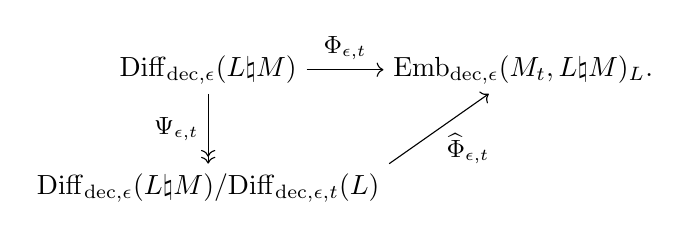
\begin{tikzpicture}
[x=1mm,y=1mm]
\node (b) at (0,0) {$\diffdece(L \natural M) / \diffdecet(L)$};
\node (t) at (0,15) {$\diffdece(L \natural M)$};
\node (r) at (40,15) {$\embdece(M_t,L\natural M)_L.$};
\draw[->>] (t) to node[left,font=\small]{$\Psi_{\epsilon,t}$} (b);
\draw[->] (t) to node[above,font=\small]{$\Phi_{\epsilon,t}$} (r);
\draw[->] (b.north east) to (r);
\node at (33,5) [font=\small] {$\widehat{\Phi}_{\epsilon,t}$};
\end{tikzpicture}
\end{center}
By definition of the right-hand embedding space, the map $\Phi_{\epsilon,t}$ is surjective, and so is the induced map $\widehat{\Phi}_{\epsilon,t}$. Moreover, if two diffeomorphisms of $\diffdece(L\natural M)$ have the same image under $\Phi_{\epsilon,t}$, their difference lies in $\diffdecet(L)$, so the induced map $\widehat{\Phi}_{\epsilon,t}$ is also injective.

We claim that it is sufficient to prove that $\Phi_{\epsilon,t}$ is a fibre bundle. Indeed, it is then a quotient map, since surjective fibre bundles are always quotient maps. Thus the induced map $\widehat{\Phi}_{\epsilon,t}$ must be a homeomorphism. This implies:
\begin{itemize}
\item[$\circ$] The map $\Psi_{\epsilon,t}$ is also a fibre bundle, hence a Serre fibration.
\item[$\circ$] Its target space is homeomorphic to the embedding space $\embdece(M_t,L\natural M)_L$, which we have given the Whitney topology, so it is Hausdorff.
\item[$\circ$] We also obtain the second statement of the proposition:
\begin{align*}
\diffdec(L \natural M) / \diffdec(L) &\cong
\underset{\epsilon,t\,\to\,0}{\colim}\left(\diffdece(L\natural M) / \diffdecet(L)\right) \\
&\cong \underset{\epsilon,t\,\to\,0}{\colim}\left(\embdece(M_t,L\natural M)_L\right) \\
&\cong \embdec(M,L\natural M)_L,
\end{align*}
by combining the identification of $\Psi \cong \underset{\epsilon,t\,\to\,0}{\colim}(\Psi_{\epsilon,t})$ with the colimit of $\widehat{\Phi}_{\epsilon,t}$ and~\eqref{eq:emb-colimit-identification}.
\end{itemize}

It therefore remains just to prove that $\Phi_{\epsilon,t}$ is a fibre bundle. Since it is equivariant with respect to the left action of $\diffdece(L\natural M)$, it suffices to prove that the action of $\diffdece(L\natural M)$ on $\embdece(M_t,L\natural M)_L$ is \emph{locally retractile}. This is because, by~\cite[Th.~A]{Palais1960Localtrivialityof}, any $G$-equivariant map into a $G$-locally retractile space is a fibre bundle.

Thus, we have to prove the following: given an embedding $e \in \embdece(M_t,L\natural M)_L$, we may find an open neighbourhood $\cU$ of $e$ and continuous map $\gamma \colon \cU \to \diffdece(L\natural M)$ such that $\gamma(e) = \id$ and $\gamma(f) \circ e = f$ for any $f \in \cU$. Note that, since $\diffdece(L\natural M)$ acts transitively on $\embdece(M_t,L\natural M)_L$ (because $\Phi_{\epsilon,t}$ is both equivariant and surjective), it suffices to prove this for just one such $e$, which we take to be the inclusion $M_t \hookrightarrow L \natural M$.

To prove this, we apply a result of Cerf~\cite[p.~291, Lem.~II.2.1.2]{Cerf1961Topologiedecertains}, which we first recall. Let $X$ be a manifold-with-corners. This means in particular that $X$ has a stratification into \emph{faces} (for example, if $X$ is a connected manifold with boundary, but no higher-codimension corners, then its set of faces is $\pi_{0}(\partial X) \sqcup \{X\}$). Each point $x \in X$ may lie in many faces, but it has a unique \emph{smallest} face (according to inclusion) in which it lies, which we denote by $\sC_{X}(x)$. Now if $Y$ is any submanifold-with-corners of $X$, we define

\begin{multline*}
C^{\infty}_{\rface}(Y,X)\\
= \{ \text{smooth maps } \varphi \colon Y \to X \text{ such that } \sC_{X}(\varphi(x)) = \sC_{X}(x) \text{ for each } x \in Y \},
\end{multline*}
equipped with the Whitney topology. The~\cite[\emph{Extension Lemma} II.2.1.2]{Cerf1961Topologiedecertains} says that, if $Y$ is closed in $X$ and $V$ is any neighbourhood of $Y$ in $X$, then the restriction map
\[
C^{\infty}_{\rface}(X,X) \too C^{\infty}_{\rface}(Y,X)
\]
admits a section $s$ defined on an open neighbourhood $\cV$ of the inclusion in $C^{\infty}_{\rface}(Y,X)$, such that $s(\rincl) = \id$ and $s(f)(x) = x$ for all $f \in \cV$ and $x \in X \smallsetminus V$.


\begin{step}{{}}
Let us write $\partial_\bullet L$ for the union of all boundary components of $L$ except for the one that intersects the image of $e_{2}$; see Figure~\ref{fig:decorated-manifolds-Mt}. Note that $\partial_\bullet L$ may or may not intersect the image of $e_{1}$. Then there is a canonical identification:
\begin{equation}\label{eq:boundary-components-identification}
\pi_{0}(\partial(L\natural M)) \cong \pi_{0}(\partial_\bullet L) \sqcup \pi_{0}(\partial M).
\end{equation}
This is necessarily asymmetric in $L$ and $M$. Each embedding $f \in \embdece(M_t,L\natural M)_L$ extends to a diffeomorphism of $L \natural M$, so it induces an injection $f_\partial \colon \pi_{0}(\partial M) \to \pi_{0}(\partial (L\natural M))$. In particular, if $f$ is the inclusion, then $f_\partial$ is also the inclusion, under the identification~\eqref{eq:boundary-components-identification}. In addition, we know that $f$ sends $B$ into $A \sqcup B$, so it also induces a map $f_\sharp \colon \pi_{0}(B) \to \pi_{0}(A) \sqcup \pi_{0}(B)$, which must be an injection since $A$ and $B$ are closed manifolds and $f$ is an embedding. The function $f \mapsto (f_\partial,f_\sharp)$ is locally constant, so its fibres are open. Let $\cU'$ be the open subset of $\embdece(M_t,L\natural M)_L$ consisting of all $f$ such that $f_\partial$ is the inclusion and $f_\sharp(\pi_{0}(B)) = \pi_{0}(B)$. Note that the second condition implies that $f(B) = B$, since $f$ is an embedding and $B$ is a closed manifold.
\end{step}

\begin{step}{{}}
Write $M_{\epsilon,t} = e_{1}(\bB_{\epsilon}^d) \sqcup M_t$ (pictured in Figure~\ref{fig:decorated-manifolds-Mepsilont}). Let
\[
\gamma' \colon \embdece(M_t,L\natural M)_L \too C^\infty(M_{\epsilon,t},L\natural M)
\]
be the continuous map that extends a given embedding $M_t \hookrightarrow L \natural M$ to a smooth map $M_{\epsilon,t} \to L \natural M$ by defining it to be the identity on $e_{1}(\bB_{\epsilon}^d)$. Note that this may fail to be injective, so it is just a smooth map, not necessarily an embedding. Also observe that, if $f$ lies in the open subset $\cU'$ from Step 1, then $\gamma'(f)$ lies in the subspace $C_{\rface}^\infty(M_{\epsilon,t},L\natural M)$, since it takes points of $\Int{(L\natural M)} \cap M_{\epsilon,t}$ into the interior of $L\natural M$ and, for any boundary component $P$ of $L\natural M$, it takes $P \cap M_{\epsilon,t}$ into $P$ (this uses the fact that $f_\partial = \id$). Restricting $\gamma'$ to $\cU'$, we therefore have a continuous map
\[
\gamma' \colon \cU' \too C^{\infty}_{\rface}(M_{\epsilon,t}, L \natural M)
\]
such that $\gamma'(\rincl) = \rincl$ and $\gamma'(f)|_{M_t} = f$ for all $f \in \cU'$.
\end{step}


\begin{step}{{}}
Now set $X = L \natural M$ and $Y = M_{\epsilon,t}$ in the Extension Lemma of Cerf above, and choose $V$ to be any open neighbourhood of $M_{\epsilon,t}$ in $L \natural M$ that is disjoint from the submanifold $A \subset \Int{L}$. Composing the local section $s$ obtained from the Extension Lemma~with $\gamma'$, we have a continuous map
\[
\gamma'' = s \circ \gamma' \colon \cU'' = (\gamma')^{-1}(\cV) \too C^{\infty}_{\rface}(L \natural M,L \natural M)
\]
such that $\gamma''(\rincl) = \id$ and for any $f \in \cU''$ we have $\gamma''(f)|_{M_t} = f$ and $\gamma''(f)(A) = A$. Moreover, by construction, we also know that $\gamma''(f)(B) = B$ and $\gamma''(f)(x) = x$ for all $x \in e_{1}(\bB_{\epsilon}^d) \sqcup e'_{2}(\bB_{\epsilon}^d)$.
\end{step}


\begin{step}{{}}
Finally, note that $\Diff(L \natural M)$ is open in $C^\infty(L\natural M,L\natural M)$, so
\[
\cU = (\gamma'')^{-1}\big(C^{\infty}_{\rface}(L \natural M,L \natural M) \cap \Diff(L\natural M)\big)
\]
is an open neighbourhood of the inclusion in $\embdece(M_t,L\natural M)_L$. For each $f \in \cU$, the diffeomorphism $\gamma''(f)$ of $L \natural M$ fixes each point of $e_{1}(\bB_{\epsilon}^d) \sqcup e'_{2}(\bB_{\epsilon}^d)$ and sends $A \sqcup B$ onto itself, so it is an element of $\diffdece(L\natural M)$. So we have a continuous map
\[
\gamma = \gamma''|_{\cU} \colon \cU \too \diffdece(L\natural M)
\]
such that $\gamma(\rincl) = \id$ and, for all $f \in \cU$, we have $\gamma(f) \circ \rincl = \gamma(f)|_{M_t} = f$.
\end{step}

%\break
\textbf{Summary.} The $4$-step construction above may be summarised in the following commutative diagram:
\begin{center}
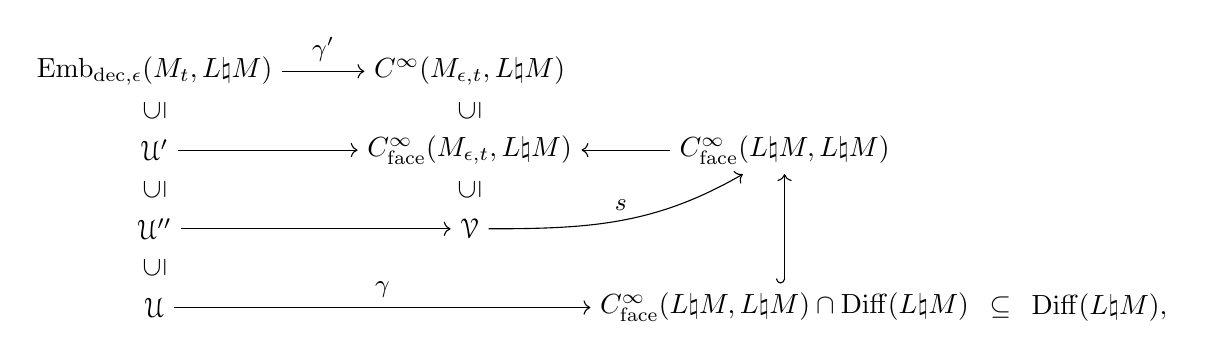
\begin{tikzpicture}
[x=1mm,y=1mm]
\node (tl) at (0,20) {$\embdece(M_t,L\natural M)$};
\node (tm) at (40,20) {$C^\infty(M_{\epsilon,t},L\natural M)$};
\node (ml) at (0,10) {$\cU'$};
\node (mm) at (40,10) {$C_{\rface}^\infty(M_{\epsilon,t},L\natural M)$};
\node (mr) at (80,10) {$C_{\rface}^\infty(L\natural M,L\natural M)$};
\node (bl) at (0,0) {$\cU''$};
\node (bm) at (40,0) {$\cV$};
\node (bbl) at (0,-10) {$\cU$};
\node (bbr) at (80,-10) {$C_{\rface}^\infty(L\natural M,L\natural M) \cap \Diff(L\natural M)$};
\node (bbrr) at (120,-10) {$\Diff(L\natural M),$};
\draw[->] (tl) to node[above,font=\small]{$\gamma'$} (tm);
\draw[->] (ml) to (mm);
\draw[->] (mr) to (mm);
\draw[->] (bl) to (bm);
\draw[->] (bm) to[out=0,in=210] node[above,font=\small]{$s$} (mr);
\draw[->] (bbl) to node[above,font=\small]{$\gamma$} (bbr);
\node at ($ (bbr.east)!0.5!(bbrr.west) $) {$\subseteq$};
\incl{(bbr)}{(mr)}
\node at (0,-5) {\rotatebox{90}{$\subseteq$}};
\node at (0,5) {\rotatebox{90}{$\subseteq$}};
\node at (0,15) {\rotatebox{90}{$\subseteq$}};
\node at (40,5) {\rotatebox{90}{$\subseteq$}};
\node at (40,15) {\rotatebox{90}{$\subseteq$}};
\end{tikzpicture}
\end{center} where the construction of $\gamma$ ensures that its image lies in $\diffdece(L\natural M) \subseteq \Diff(L\natural M)$.
\end{proof}

\begin{figure}[!htbp]
\centering
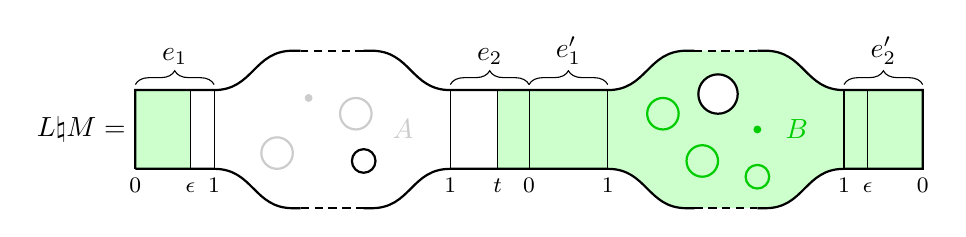
\begin{tikzpicture}
[x=1mm,y=1mm,scale=1]
\begin{scope}[xshift=5mm]
\fill[green!20] (0,0) -- (7,0) -- (7,10) -- (0,10) -- cycle;
\end{scope}
\begin{scope}[xshift=55mm]
\fill[green!20] (-4,0) -- (10,0).. controls (15,0) and (15,-5).. (20,-5) -- (21,-5) -- (29,-5) -- (30,-5).. controls (35,-5) and (35,0).. (40,0) -- (50,0) -- (50,10) -- (40,10).. controls (35,10) and (35,15).. (30,15) -- (29,15) -- (21,15) -- (20,15).. controls (15,15) and (15,10).. (10,10) -- (-4,10) -- cycle;
\end{scope}
\begin{scope}[xshift=5mm]
\draw[thick] (0,0) -- (10,0).. controls (15,0) and (15,-5).. (20,-5) -- (21,-5);
\draw[thick,densely dashed] (21,-5) -- (29,-5);
\draw[thick] (29,-5) -- (30,-5).. controls (35,-5) and (35,0).. (40,0) -- (50,0);
\draw[thick] (50,10) -- (40,10).. controls (35,10) and (35,15).. (30,15) -- (29,15);
\draw[thick,densely dashed] (29,15) -- (21,15);
\draw[thick] (21,15) -- (20,15).. controls (15,15) and (15,10).. (10,10) -- (0,10) -- (0,0);
\draw[black!20,thick] (18,2) circle (2);
\draw[black!20,thick] (28,7) circle (2);
\fill[black!20,thick] (22,9) circle (0.5);
\node at (34,5) [black!20] {$A$};
\fill[white] (29,1) circle (1.5);
\draw[thick] (29,1) circle (1.5);
\draw (7,0) -- (7,10);
\draw (10,0) -- (10,10);
\node at (0,0) [anchor=north,font=\footnotesize] {$0$};
\node at (7,0) [anchor=north,font=\footnotesize] {$\vphantom{0}\epsilon$};
\node at (10,0) [anchor=north,font=\footnotesize] {$1$};
\node at (5,12) [anchor=south] {$e_{1}$};
\draw[decorate,decoration={brace,amplitude=5pt,raise=2pt}] (0,10) -- (10,10);
\node at (0,5) [anchor=east] {$L \natural M =$};
\end{scope}
\begin{scope}[xshift=55mm]
\draw[thick] (0,0) -- (10,0).. controls (15,0) and (15,-5).. (20,-5) -- (21,-5);
\draw[thick,densely dashed] (21,-5) -- (29,-5);
\draw[thick] (29,-5) -- (30,-5).. controls (35,-5) and (35,0).. (40,0) -- (50,0) -- (50,10) -- (40,10).. controls (35,10) and (35,15).. (30,15) -- (29,15);
\draw[thick,densely dashed] (29,15) -- (21,15);
\draw[thick] (21,15) -- (20,15).. controls (15,15) and (15,10).. (10,10) -- (0,10);
\draw[green!80!black,thick] (17,7) circle (2);
\draw[green!80!black,thick] (22,1) circle (2);
\draw[green!80!black,thick] (29,-1) circle (1.5);
\fill[green!80!black,thick] (29,5) circle (0.5);
\fill[white] (24,9.5) circle (2.5);
\draw[thick] (24,9.5) circle (2.5);
\node at (34,5) [green!80!black] {$B$};
\draw (40,0) -- (40,10);
\draw (43,0) -- (43,10);
\node at (40,0) [anchor=north,font=\footnotesize] {$1$};
\node at (43,0) [anchor=north,font=\footnotesize] {$\vphantom{0}\epsilon$};
\node at (50,0) [anchor=north,font=\footnotesize] {$0$};
\node at (45,12) [anchor=south] {$e'_{2}$};
\draw[decorate,decoration={brace,amplitude=5pt,raise=2pt}] (40,10) -- (50,10);
\draw (-10,0) -- (-10,10);
\draw (-4,0) -- (-4,10);
\draw (0,0) -- (0,10);
\draw (10,0) -- (10,10);
\node at (-10,0) [anchor=north,font=\footnotesize] {$1$};
\node at (-4,0) [anchor=north,font=\footnotesize] {$\vphantom{0}t$};
\node at (0,0) [anchor=north,font=\footnotesize] {$0$};
\node at (10,0) [anchor=north,font=\footnotesize] {$1$};
\draw[decorate,decoration={brace,amplitude=5pt,raise=2pt}] (-10,10) -- (0,10);
\draw[decorate,decoration={brace,amplitude=5pt,raise=2pt}] (0,10) -- (10,10);
\node at (-5,12) [anchor=south] {$e_{2}$};
\node at (5,12) [anchor=south] {$e'_{1}$};
\end{scope}
\end{tikzpicture}
\caption{The submanifold $M_{\epsilon,t}$ (shaded in green) of $L \natural M$ from the proof of Theorem~\ref{thm:fibre-bundle}.}\label{fig:decorated-manifolds-Mepsilont}
\end{figure}

\begin{thebibliography}{99}
\bibitem[Cer61]{Cerf1961Topologiedecertains} Jean Cerf, ``Topologie de certains espaces de plongements'', \emph{Bull. Soc. Math. Fr.} \textbf{89} (1961), 227--380.
\bibitem[Pal60b]{Palais1960Localtrivialityof} R. S. Palais, ``Local triviality of the restriction map for embeddings'', \emph{Comment. Math. Helv.} \textbf{34} (1960), 305--312.
\bibitem[Lim63]{Lima1963localtrivialityof} Elon L. Lima, ``On the local triviality of the restriction map for embeddings'', \emph{Comment. Math. Helv.} \textbf{38} (1963), 163--164.
\bibitem[Hir76]{Hirsch1976Differentialtopology} Morris W. Hirsch, \emph{Differential topology}, Graduate Texts in Mathematics, vol. 33, Springer, 1976.
\bibitem[MMSS01]{MMSS} Michael A. Mandell, Jon P. May, Stefan Schwede, and Brooke E. Shipley, ``Model categories of diagram spectra'', \emph{Proc. Lond. Math. Soc.} \textbf{82} (2001), no. 2, 441--512.
\bibitem[TV08]{ToenVezzosi} Bertrand To\"en and Gabriele Vezzosi, ``Homotopical algebraic geometry. II. Geometric stacks and applications'', \emph{Mem. Am. Math. Soc.} \textbf{193} (2008), no. 902.
\bibitem[Bro60]{Brown1960} Morton Brown, ``A proof of the generalized Schoenflies theorem'', \emph{Bull. Am. Math. Soc.} \textbf{66} (1960), 74--76.
\bibitem[Mat69]{Mather1969} John N. Mather, ``Stability of $C^\infty$ mappings. II. Infinitesimal stability implies stability'', \emph{Ann. Math.} \textbf{89} (1969), 254--291.
\bibitem[Maz59]{Mazur1959} Barry Mazur, ``On embeddings of spheres'', \emph{Bull. Am. Math. Soc.} \textbf{65} (1959), 59--65.
\bibitem[Mil65]{Milnor1965} John Milnor, \emph{Lectures on the $h$-cobordism theorem}, Princeton University Press, 1965, notes by L. Siebenmann and J. Sondow.
\bibitem[Mor60]{Morse1960} Marston Morse, ``A reduction of the Schoenflies extension problem'', \emph{Bull. Am. Math. Soc.} \textbf{66} (1960), 113--115.
\bibitem[Pal60a]{Palais1960Extendingdiffeomorphisms} Richard S. Palais, ``Extending diffeomorphisms'', \emph{Proc. Am. Math. Soc.} \textbf{11} (1960), 274--277.
\bibitem[Sch06]{Schoenflies1906} Arthur M. Schoenflies, ``Beitr\"age zur Theorie der Punktmengen. III'', \emph{Math. Ann.} \textbf{62} (1906), no. 2, 286--328.
\end{thebibliography}
\end{document}
